% !TEX TS-program = pdflatex
% !TEX encoding = UTF-8 Unicode

%\documentclass[a4paper,twoside]{article}%                                        use larger type; default would be 10pt
\documentclass[a4paper,draft]{article}%                                                 use larger type; default would be 10pt
\usepackage[utf8]{inputenc}%                                                      set input encoding (not needed with XeLaTeX)

%%% PAGE DIMENSIONS ------------------------------------------------------------
\usepackage{geometry}%              to change the page dimensions
\geometry{a4paper}%                                                               or letterpaper (US) or a5paper or....
\usepackage[parfill]{parskip}%                                                    Activate to begin paragraphs with an empty line rather than an indent

%%% HEADERS & FOOTERS ----------------------------------------------------------
\usepackage{fancyhdr}%                                                            This should be set AFTER setting up the page geometry
\pagestyle{fancy}%                                                                options: empty , plain , fancy
\renewcommand{\headrulewidth}{0pt}%                                               customise the layout...
\lhead{}\chead{}\rhead{}
\lfoot{}\cfoot{page \thepage}\rfoot{}

%%% SECTION TITLE APPEARANCE ---------------------------------------------------
%\usepackage{sectsty}
%\allsectionsfont{\sffamily\mdseries\upshape}%                                     (See the fntguide.pdf for font help)

%%% PACKAGES -------------------------------------------------------------------
%\usepackage{morefloats}
\usepackage[font=small,labelfont=bf,textfont=it]{caption}%                        stylize captions
\usepackage[pdftex]{graphicx}%                                                    support the \includegraphics command and options
\usepackage{booktabs}%                                                            for much better looking tables
\usepackage{array}%                                                               for better arrays (eg matrices) in maths
%\usepackage{paralist}%                                                            very flexible & customisable lists (eg. enumerate/itemize, etc.)
\usepackage{verbatim}%                                                            adds environment for commenting out blocks of text & for better verbatim
%\usepackage{subfig}%                                                              make it possible to include more than one captioned figure/table in a single float
\usepackage{subcaption}
\usepackage{mathtools}%                                                           for math environments like align
\usepackage{amssymb}%                                                             for symbols like \therefore
\usepackage{verbatim}%                                                            for including text as appears, verbatim
\usepackage{listings}%                                                            for including external files as text, eg code
\usepackage{color}%                                                               for coloring of files and images
%\usepackage{overpic}%                                                             for adding annotations to pictures
%\usepackage{multirow}%                                                            for multiple row spanning cells in tables
\usepackage{rotating}%                                                            for the \begin{sideways} environment for sideways text

%% BIBIOGRAPHY ------------------------------------------------------------------
\usepackage{cite}

%%% ToC (table of contents) APPEARANCE -----------------------------------------
%\usepackage[nottoc,notlof,notlot]{tocbibind}                                   % Put the bibliography in the ToC
%\usepackage[titles,subfigure]{tocloft}                                         % Alter the style of the Table of Contents
%\renewcommand{\cftsecfont}{\rmfamily\mdseries\upshape}
%\renewcommand{\cftsecpagefont}{\rmfamily\mdseries\upshape}                     % No bold!
\setcounter{tocdepth}{2}

%%% PDF LINKS AND STYLE --------------------------------------------------------
\usepackage[unicode=true,
    bookmarks=true,bookmarksnumbered=true,bookmarksopen=true,
    bookmarksopenlevel=2, breaklinks=false,pdfborder={0 0 0},backref=false,
    colorlinks=false] {hyperref}%                                                 for links in pdf file, no colors
\hypersetup{pdftitle={Human Computer Interaction},
    pdfauthor={}}%    set name of document and author here

%%% END Article customizations

%*******************************************************************************
%******************************** END HEADER ***********************************
%*******************************************************************************

\begin{document}
%!TEX root = mainfile.tex
\begin{titlepage}
	\begin{center}
	\vspace*{\fill}

	\centering
	
\includegraphics[scale=1.0]{Logo.pdf}
	\vfill

	\hrule
	{\LARGE\bf Human Computer Interaction \\
		--- \\
		Unified Sports Booking System\\[0.4cm]}
	\hrule

	\vfill
	% \large
	% School of Computer Science\\
	% University of Birmingham

	\vfill
		Rebecca Devney,\\
		Assima Pathan,\\
		Josh Wainwright,\\
		Andrew Walker
	\vfill
		\textbf{Group 5}
	\vfill

	\vfill
	\textit{Supervisor:} Robert Henley \\
	\vfill
	\textit{Date:} March 2014
	\vfill
	\vfill

	\begin{abstract}
		If you currently want to book sports facilities, the only way to search
		is directly through the individual sports center's websites, or through
		direct communication. If someone is flexible in the location or choice
		of sport, they are required to search multiple locations to find the
		best compromise.

		In addition to the difficulties of checking multiple websites, often
		each of these websites are unintuitive and difficult to use, requiring
		the user to know exactly when and where they want to use the facilities
		and often not giving clear information about other possible factors
		such as cost.

		Here, we propose a new, unified interface for finding a time, location
		and the cost for playing any of a number of sports, at any of the
		available locations within a given distance or relative to a different
		location.
	\end{abstract}

	\end{center}
\end{titlepage}

%\thispagestyle{empty}
%\vspace*{\fill}
%\noindent
%\begin{tabular}{ll}
%\end{tabular}

%\cleardoublepage
%\cleardoublepage

\newpage
\tableofcontents
\addcontentsline{toc}{section}{Contents}
\newpage

\section{Review of Related Work}
\label{sec:review_of_related_work}

\subsection{User Input}
\label{sub:user_input}

In order to present a user with useful information, our application will have
to accept data from them. This is done by means of forms, text input and
buttons. To maintain a clean, intuitive user interface, a simplistic approach
is often taken to reduce the thinking time required to process information on a
single screen. If more information is required, multiple screens are often
used.

\subsubsection{Timetables}
\label{ssub:timetables}

A common set of information presented to a user which represents a considerable
challenge, particularly on small screens, is a timetable of available or
appropriate times. From this, the user can then select which is most suitable
for them. When too much information is displayed on a single screen, this can
become confusing or impossible to read. For example, in
figure~\ref{fig:GoogleCalendarTimetable}\cite{GoogleCalendar}, despite a single
hour being a common appointment length, the text for these slots is hidden
entirely.
\begin{figure}[ht]
	\centering
	\begin{subfigure}[b]{0.25\textwidth}
		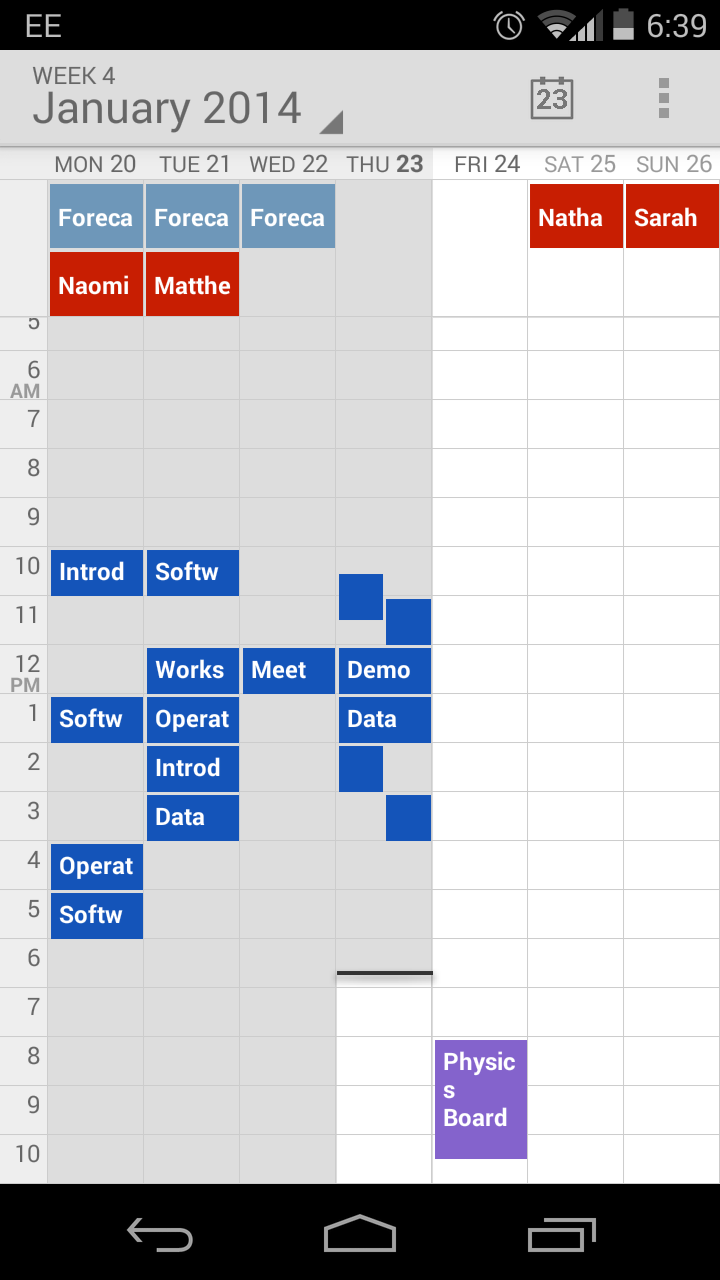
\includegraphics[width=\textwidth]{img/relatedReviews/GoogleCalendarTimetable.png}
		\caption{Google Calendar}\label{fig:GoogleCalendarTimetable}
	\end{subfigure}%
	\qquad
	\begin{subfigure}[b]{0.25\textwidth}
		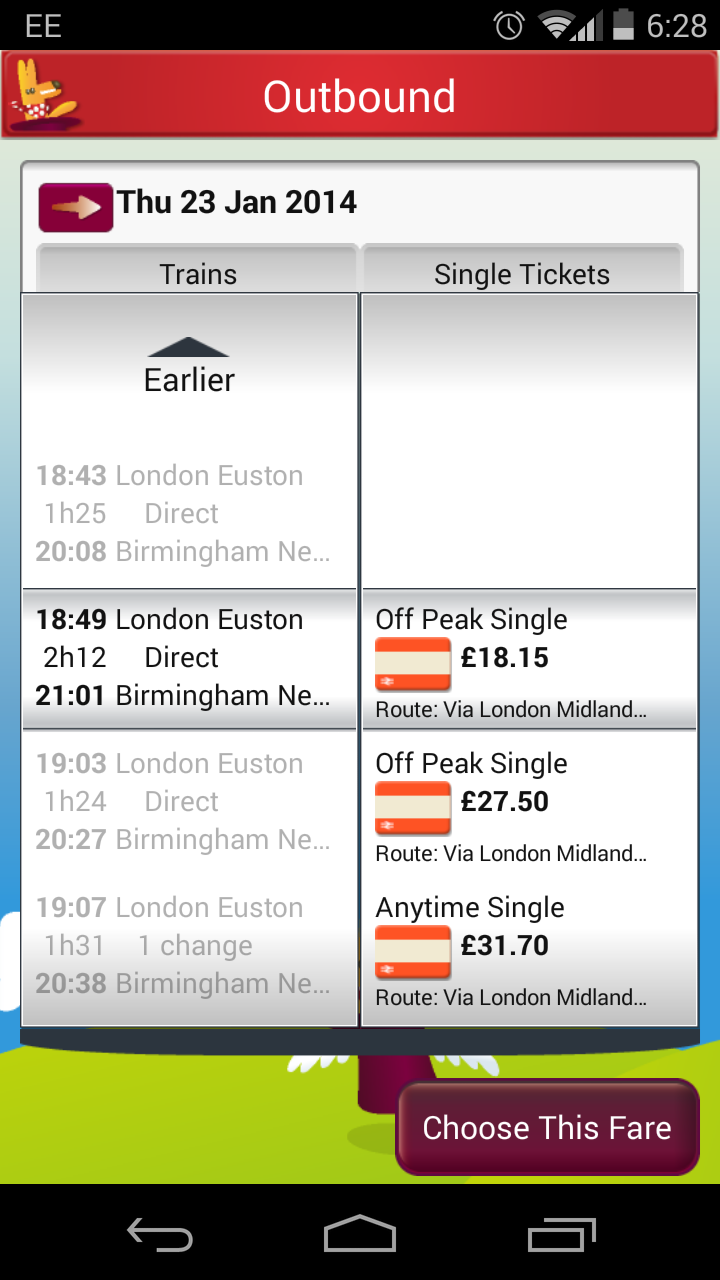
\includegraphics[width=\textwidth]{img/relatedReviews/RedSpottedHankyTicketSelection}
		\caption{RedSpottedHanky}\label{fig:RedSpottedHankyTicketSelection}
	\end{subfigure}
	\caption{When too much information is displayed on a screen, it can be
		hard to read and interpret, whereas condensing the information and
		splitting it so that only currently appropriate information is shown
	makes it much easier to understand. }\label{fig:timetables}
\end{figure}

A common way to improve the readability of theses complex structures, which
often contain a large quantity of data, is to have graded selection of that
data. In other words, where there is an option to refine a search to reduce the
data needed to be displayed, only the  immediately relevant information is
displayed, with simple navigation to other relevant data.

This method can be seen clearly in the RedSpottedHanky.com application,
figure~\ref{fig:RedSpottedHankyTicketSelection} when a user is searching for
tickets for a specific date and time. Although there may be many trains within
a narrow time gap, the application shows a small number of tickets with the
option to move either earlier or later. Each ticket time is also associated
with a number of options relating to ticket price. These are shown only for the
currently selected ticket time.

% subsubsection timetables (end)

\subsubsection{Date/Time Selection}
\label{ssub:date_time_selection}

In order to reduce the search range, often a date and/or time selection
dialogue is used. Figure~\ref{fig:date_time_selection} shows two different
implementations.

Figure~\ref{fig:RedSpottedHankyDateTime}, on the right is an example, again,
from RedSpottedHanky\cite{RedSpottedHanky}, which shows the time selection
associated with booking a train ticket. This design fails since the method of
changing time requires very close control when accuracy is required, and is
time consuming when the desired time is far from the currently selected time.
The movement is performed in single increments or decrements of the hours and
minutes. This is despite the functionality described above which lets the user
view and switch to other trains at nearby times.

Figures~\ref{fig:GoogleCalendarDateTime}, in the middle
and~\ref{fig:GoogleCalendarDateTime2} on the left are examples from Google
Calendar which shows how the process can be made much more intuitive, simple
and fast. Through the use of separate screens with large and clear selection,
this selection is much easier to navigate than the scrolling method used above.
\begin{figure}[ht]
	\centering
	\begin{subfigure}[b]{0.25\textwidth}
		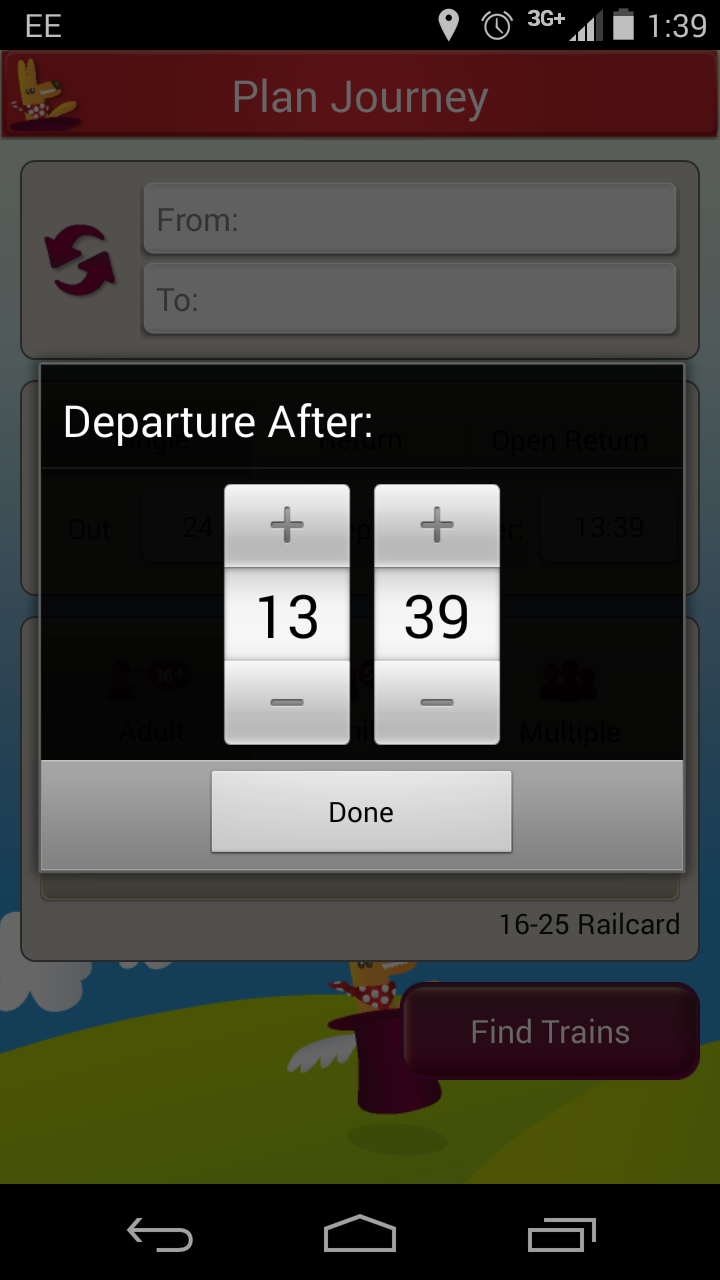
\includegraphics[width=\textwidth]{img/relatedReviews/RedSpottedHankyDateTime}
		\caption{RedSpottedHanky}\label{fig:RedSpottedHankyDateTime}
	\end{subfigure}%
	\qquad
	\begin{subfigure}[b]{0.25\textwidth}
		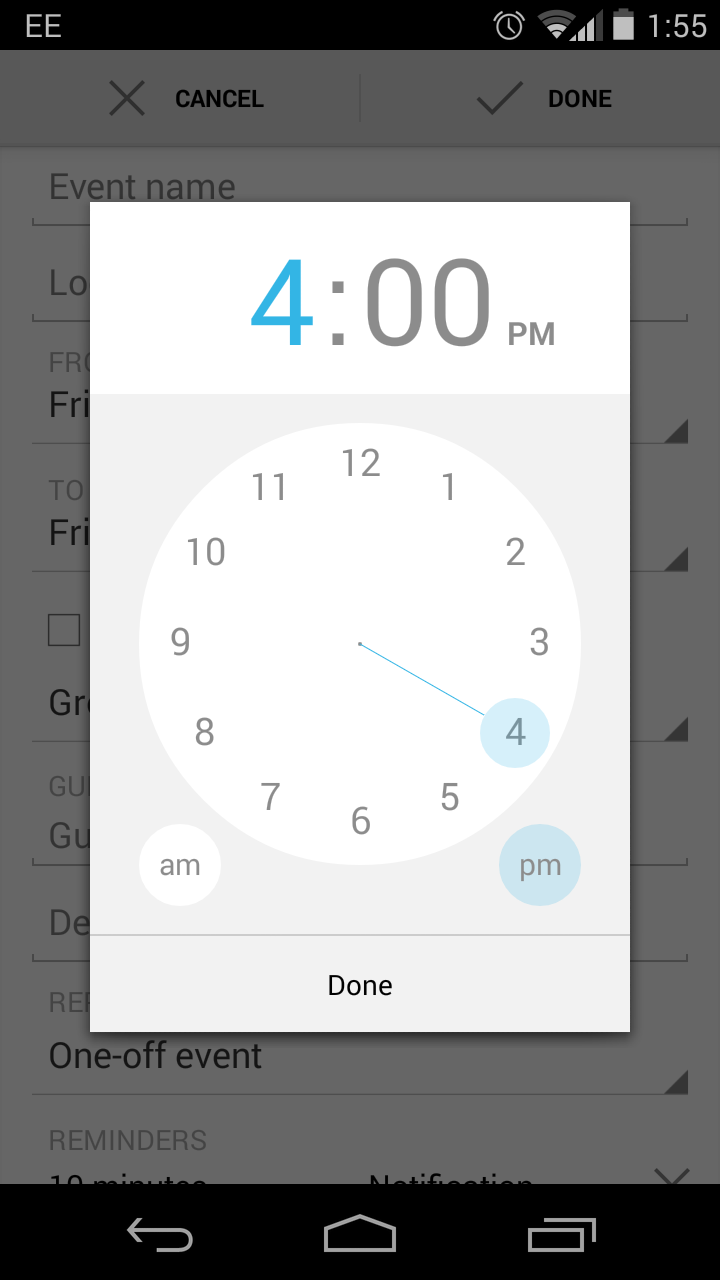
\includegraphics[width=\textwidth]{img/relatedReviews/GoogleCalendarDateTime}
		\caption{Google Calendar}\label{fig:GoogleCalendarDateTime}
	\end{subfigure}
	\qquad
	\begin{subfigure}[b]{0.25\textwidth}
		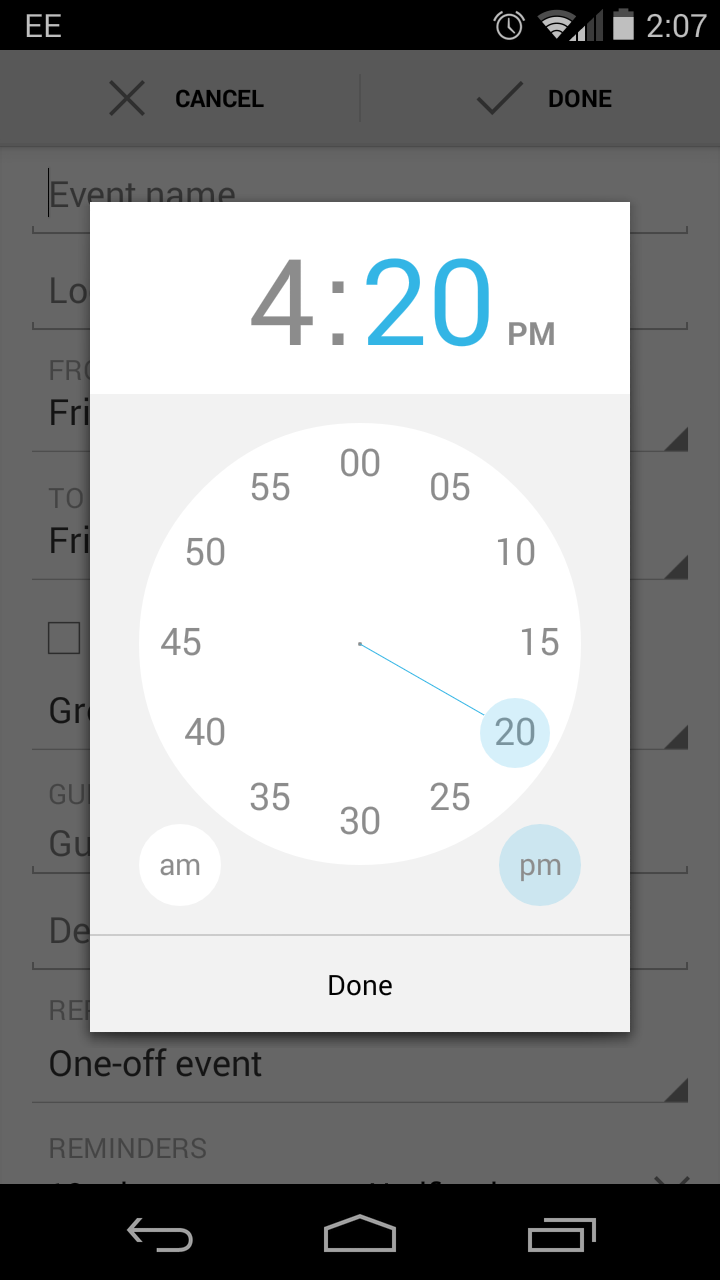
\includegraphics[width=\textwidth]{img/relatedReviews/GoogleCalendarDateTime2}
		\caption{Google Calendar}\label{fig:GoogleCalendarDateTime2}
	\end{subfigure}
	\caption{The time selection for RedSpottedHanky requires the user to
		spend to much time selecting the time when larger increments could be
		used to smoothen the process. Google Calendar, on the other hand,
		allows simple and fast selection of the hours and minutes through
	separate screens. }\label{fig:date_time_selection}
\end{figure}

A combination of both of these is used in the stock iOS, shown in
figure~\ref{fig:iOSDateTime}\cite{iOSDateTime} where a much easier to navigate
scrolling mechanism is used. Though this can still cause the user to spend more
time selecting the correct number, the fact that the used can ``flick scroll''
though the numbers means reaching a value that is far from the currently
selected one is much quicker than the RedSpottedHanky.com application.
\begin{figure}[ht]
	\centering
	\begin{subfigure}[b]{0.25\textwidth}
		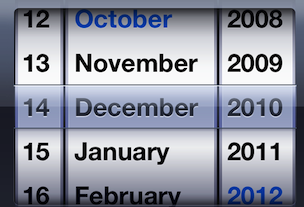
\includegraphics[width=\textwidth]{img/relatedReviews/iOSDateTime}
		\caption{RedSpottedHanky}
	\end{subfigure}%
	\qquad
	\begin{subfigure}[b]{0.35\textwidth}
		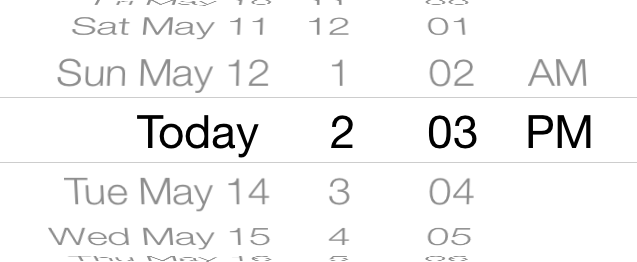
\includegraphics[width=\textwidth]{img/relatedReviews/iOS7DateTime}
		\caption{Google Calendar}
	\end{subfigure}
	\caption{Stock iOS date and time picker is easier to scroll through, but
		still requires more time than selecting the appropriate number.
	}\label{fig:iOSDateTime}
\end{figure}

% subsubsection date_time_selection (end)

\subsubsection{Forms}
\label{ssub:forms}

When entering information that is not limited to a small set of possible
values, such as a name, location or arbitrary number, a form must be used to
accept the user input. Since touch screens rely of the user being able to
navigate to to correct form section, the input must be of sufficient size to
allow this movement easily.

Figure~\ref{fig:TescoFormInput} show a simple form with two input boxes. Each
has a clear border around it so the target for interaction is easier to select.

An important consideration that has been made here is to specify that, for the
second set of text input, the data is strictly limited to digits. For this
reason, the keyboard switches from a general purpose ``qwerty'' keyboard to a
purely numerical version. Again, this assists the user, both by indicating that
only the provided digits are acceptable, and making the input of those digits
easier (often the numbers on a touch screen keyboard are only accessible by
switching modes).
\begin{figure}[ht]
	\centering
	\begin{subfigure}[b]{0.2\textwidth}
		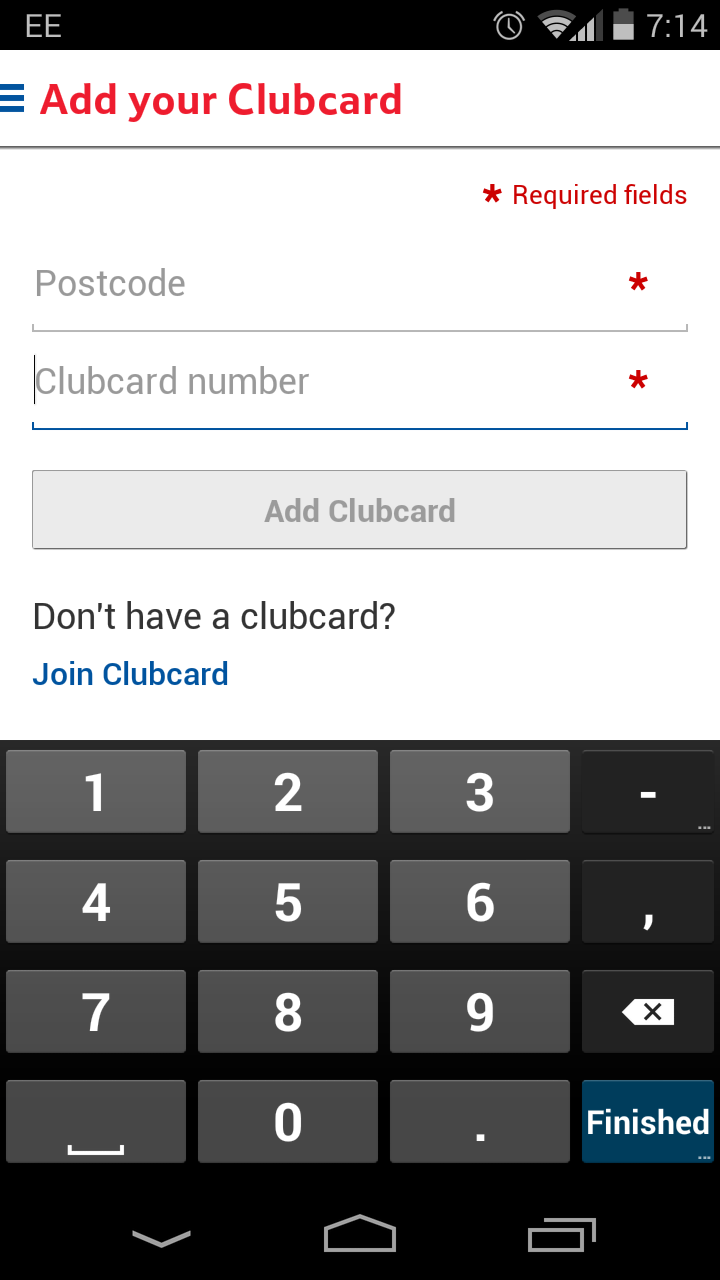
\includegraphics[width=\textwidth]{img/relatedReviews/TescoFormInput}
		\caption{Large, easy to access text entry}\label{fig:TescoFormInput}
	\end{subfigure}%
	\qquad
	\begin{subfigure}[b]{0.25\textwidth}
		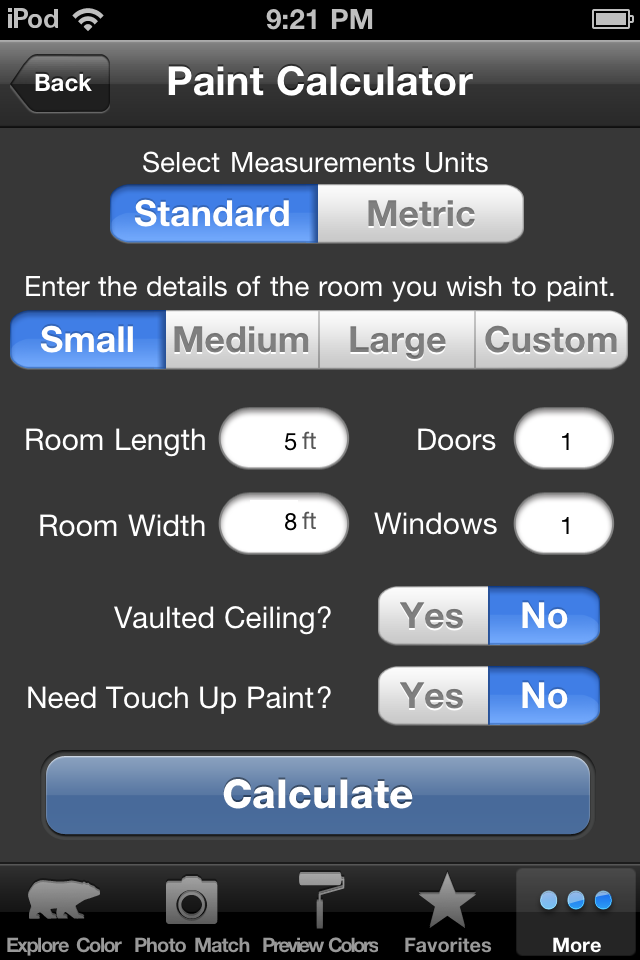
\includegraphics[width=\textwidth]{img/relatedReviews/PaintCalculatorCrowded}
		\caption{Crowded interfaces make entry more difficult.}
	\end{subfigure}
	\caption{}\label{fig:PaintCalculatorCrowded}
\end{figure}

By contrast, the interface in figure~\ref{fig:PaintCalculatorCrowded} is overly
crowded with too many small buttons squashed together. This could cause the
user to select the wrong input area, or not be able to navigate the application
properly.
% subsubsection forms (end)

% subsection user_input (end)

\subsection{Current Comparison/Booking Applications}
\label{sub:current_comparison_applications}

The idea of comparing various services to match your requirements at the best
price is widely spread over the web, especially when it comes to booking
flights, hotels, transport etc.  We want to take this idea and apply it
specifically to booking sports facilities across the county.  Some applications
compare results from different websites; others show available options from
different companies on their own website.

\subsubsection{Skyscanner}
\label{ssub:skyscanner}

Skyscanner is a flight search app which compares flights and airlines. The app
allows the user to search by airport, departure/return date, number of
passengers and cabin class. They are then directed to search results matching
their criteria. Once the user has chosen their desired flight, they are linked
to the airline or travel agent to buy directly.

% \begin{figure}[htbp]
% 	\centering
% 	\begin{subfigure}[b]{0.2\textwidth}
% 		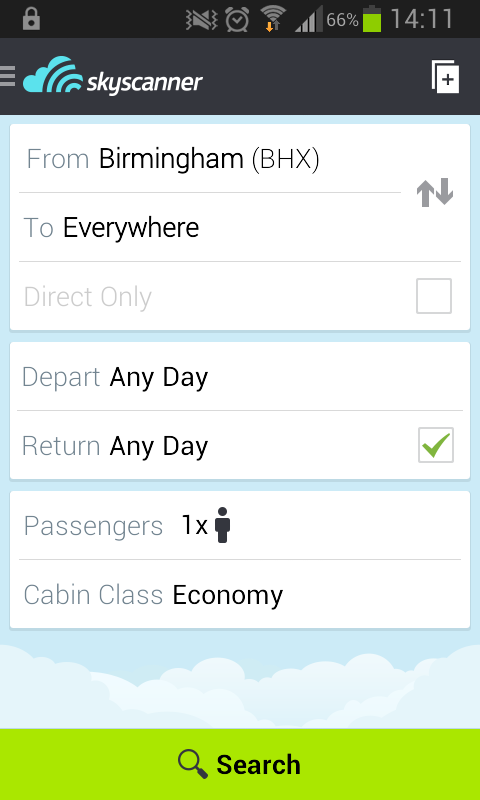
\includegraphics[width=\textwidth]{img/relatedReviews/SkyscannerFig1.png}
% 		\caption{Skyscanner's home screen}\label{fig:skyscannerfig1}
% 	\end{subfigure}%
% 	\qquad
% 	\begin{subfigure}[b]{0.2\textwidth}
% 		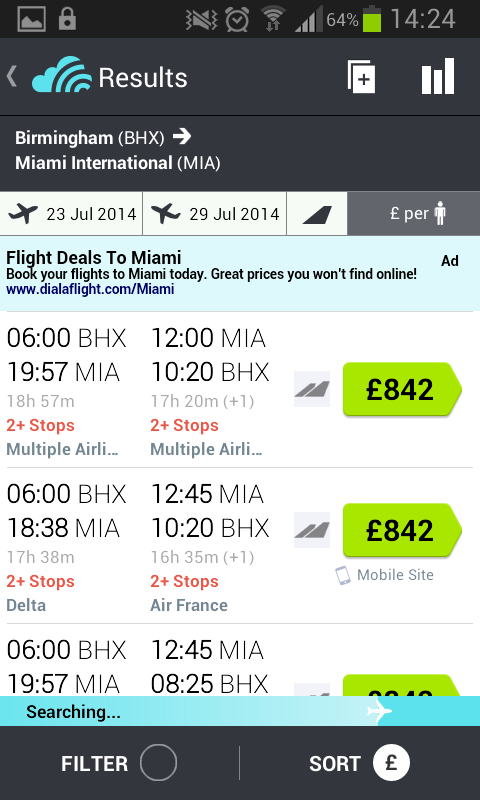
\includegraphics[width=\textwidth]{img/relatedReviews/SkyscannerFig2.png}
% 		\caption{Skyscanner's search results.}
% 	\end{subfigure}
% 	\caption{}\label{fig:skyscanner1}
% \end{figure}

\marginFig[0.8]{img/relatedReviews/SkyscannerFig2.png}{Skyscanner's search results
}{fig:skyscannerfig2}
\paragraph{Strengths}
\begin{itemize}
	\item The date selection page is simplistic and easy to use. The user is
		provided with a calendar where they can simply touch the date they
		would like to fly (figure~\ref{fig:skyscannerfig3}).
	\item Clear, concise information is shown on the results page. This allows
		the user to quickly scan the flights available and doesn't clutter the
		page with information which would not affect most customers' decisions
		(figure~\ref{fig:skyscannerfig2}). Further details (destinations and times
		of any stops) can be viewed by clicking on the flight.
	\item If a return date is not specified, an extra screen is displayed which
		allows the user to see the prices of different departure dates and the
		return dates available. This gives the customer an opportunity to
		change their departure date based on the prices shown.
		(figure~\ref{fig:skyscannerfig5})
	\item There is a filter option on the results page permitting users to be
		more specific. For example, particular airlines, direct flights only,
		flights times etc. (figure~\ref{fig:skyscannerfig4})
\end{itemize}
\begin{figure}[htbp]
	\centering
	\begin{subfigure}[b]{0.28\textwidth}
		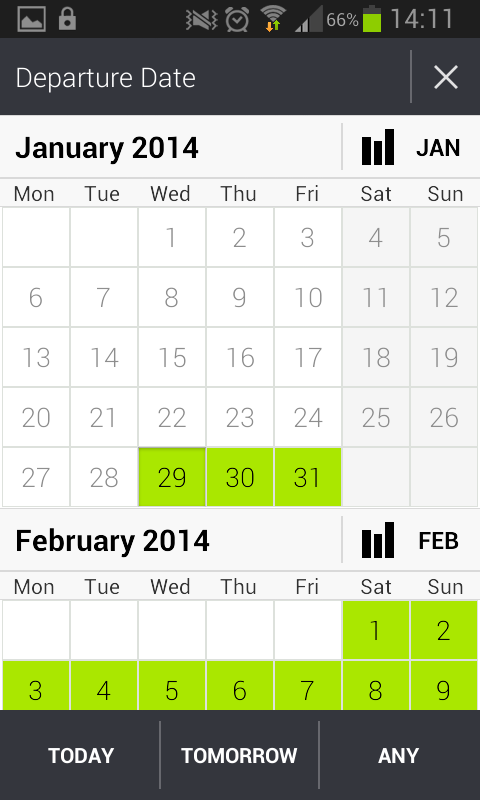
\includegraphics[width=\textwidth]{img/relatedReviews/SkyscannerFig3.png}
		\caption{Skyscanner's easy to use calendar for date selection.
		}\label{fig:skyscannerfig3}
	\end{subfigure}
	\qquad
	\begin{subfigure}[b]{0.28\textwidth}
		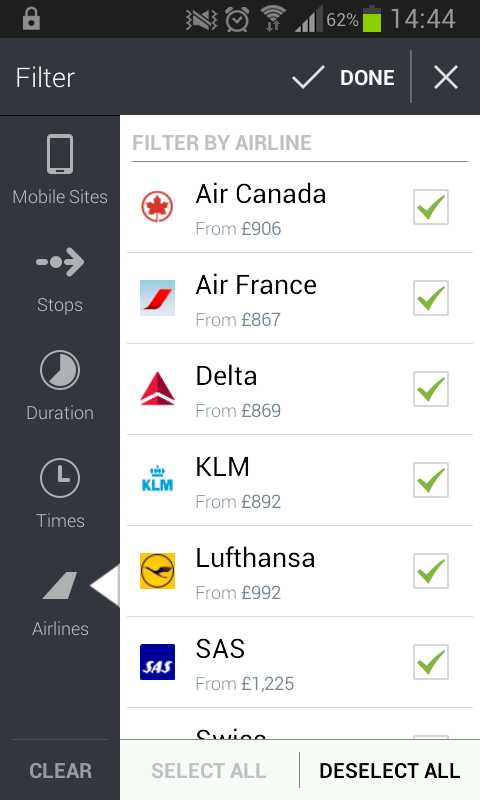
\includegraphics[width=\textwidth]{img/relatedReviews/SkyscannerFig4.png}
		\caption{Options available to further filter search results.
		}\label{fig:skyscannerfig4}
	\end{subfigure}
	\qquad
	\begin{subfigure}[b]{0.28\textwidth}
		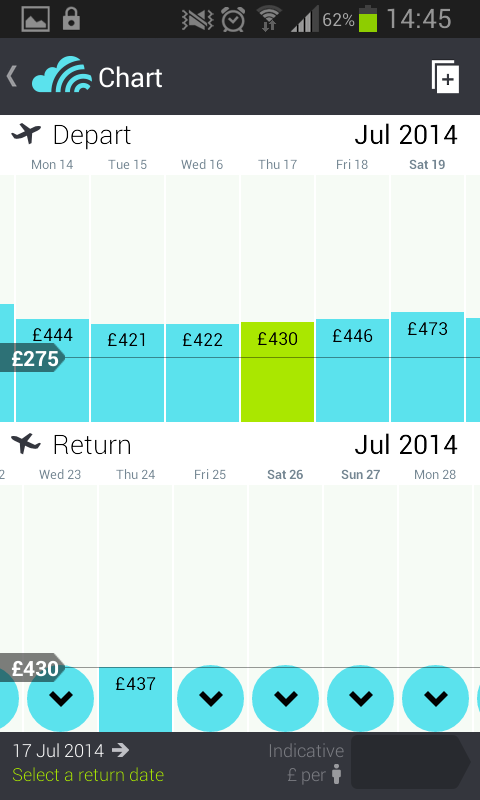
\includegraphics[width=\textwidth]{img/relatedReviews/SkyscannerFig5.png}
		\caption{Screen shows prices of alternative dates.
		}\label{fig:skyscannerfig5}
	\end{subfigure}
	\caption{}\label{fig:skyscanner2}
\end{figure}

\marginFig[0.8]{img/relatedReviews/SkyscannerFig1.png}{Skyscanner's home screen
}{fig:skyscannerfig1}
\paragraph{Weaknesses}
\begin{itemize}
	\item There is no flexibility in departure date (except for the option of
		``any'' date). However the return date option allows flexibility of one
		day.
	\item The ``Everywhere'' option (figure~\ref{fig:skyscannerfig1}) seems
		slightly pointless as it is unlikely someone would have no preference
		as to where they wish to go but have a particular date in mind. It is
		more likely they have a general idea of where they want to go, for
		example the country, but there is no option for this.
	\item When choosing a destination, the user is required to select a
		specific airport. This restricts the user to where they can fly. For
		example, they may wish to check prices to a variety of destinations
		within a particular area or group of Islands with various airports.
\end{itemize}

\subsubsection{Trivago}
\label{ssub:trivago}

Trivago is a hotel comparison website comparing hotels from booking sites such
as booking.com and Lastminute.com. The initial search screen boasts many
options and filters. As well as the expected search criteria such as location
and check in/out date, the user can also filter by rating, popularity,
distance, price and whether the hotel has certain features such as WiFi and a
pool etc. A maximum price and distance can also be set within a certain range
using the sliding bars (figures~\ref{fig:trivago1} and~\ref{fig:trivago1b}).
The results show the cheapest price for each hotel available and what booking
website the customer can get this price. Once the customer has chosen their
hotel, they will be directed to the booking website where they will make the
payment.
\marginFig[0.8]{img/relatedReviews/TrivagoFig1a.png}{Top half}{fig:trivago1}
\marginFig[0.8]{img/relatedReviews/TrivagoFig1b.png}{Bottom half}{fig:trivago1b}
% \begin{figure}[htbp]
% 	\centering
% 	\begin{subfigure}[b]{0.2\textwidth}
% 		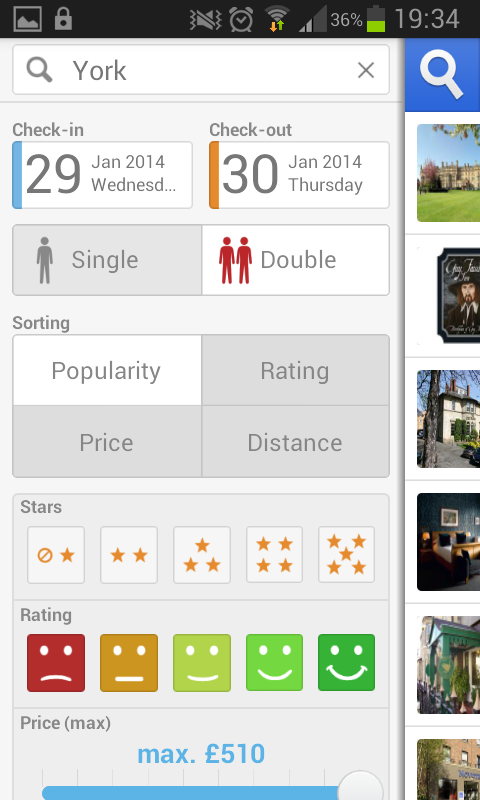
\includegraphics[width=\textwidth]{img/relatedReviews/TrivagoFig1a.png}
% 		\caption{Top half}
% 	\end{subfigure}
% 	\qquad
% 	\begin{subfigure}[b]{0.2\textwidth}
% 		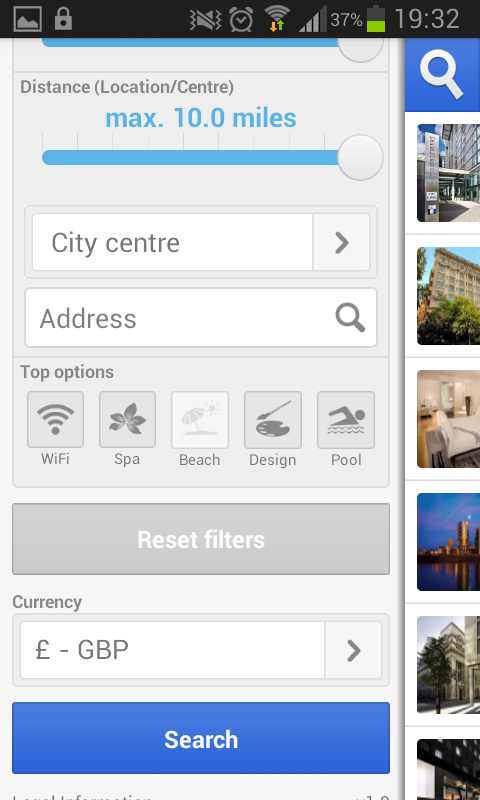
\includegraphics[width=\textwidth]{img/relatedReviews/TrivagoFig1b.png}
% 		\caption{Bottom half}
% 	\end{subfigure}
% 	\caption{Trivago's home screen}\label{fig:trivago1}
% \end{figure}

%TrivagoFig1a.png(home screen top half) TrivagoFig1b.png( home screen bottom half)

\paragraph{Strengths}
\begin{itemize}
	\item As a location is typed, the number of available hotels is displayed
		in brackets next to suggested locations.
	\item Searching is very flexible, for example you can search by hotel name,
		region, points of interest and city.
	\item It is possible to search for hotels in the vicinity of a specific
		address, very useful if you want to find the nearest hotel to a
		specific location.
	\item Search results automatically load up at the side of the screen as
		search criteria is filled out. The user can swipe across to see them,
		for example once a location had been entered, it will load up available
		hotels whilst still maintaining the search screen.
	\item The search results are very clear and simple in that they show enough
		information without clogging up the screen. The hotel name, rating,
		stars, distance from the centre, price and a photo are all displayed in
		a concise manner (figure~\ref{fig:TrivagoFig2}). The user can then look
		into more detail by clicking on the hotel
		(figure~\ref{fig:TrivagoFig3}).
\end{itemize}
\begin{figure}[htbp]
	\centering
	\begin{subfigure}[b]{0.33\textwidth}
		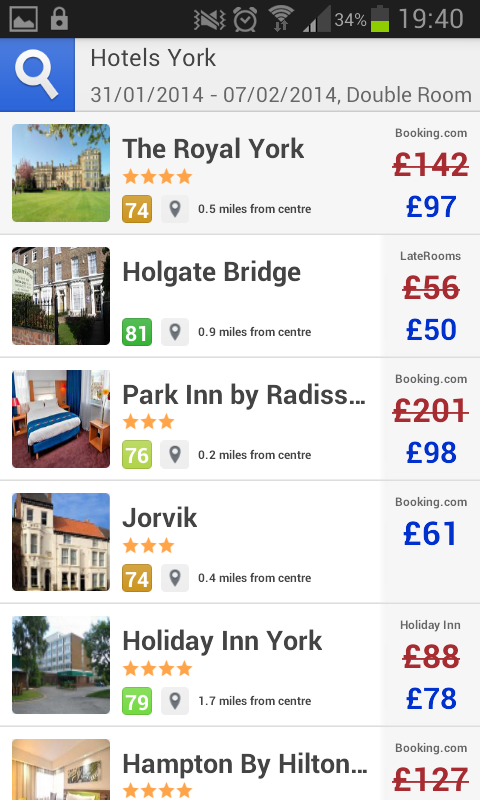
\includegraphics[width=\textwidth]{img/relatedReviews/TrivagoFig2.png}
		\caption{Trivago's earch results screen}\label{fig:TrivagoFig2}
	\end{subfigure}%
	\qquad
	\begin{subfigure}[b]{0.33\textwidth}
		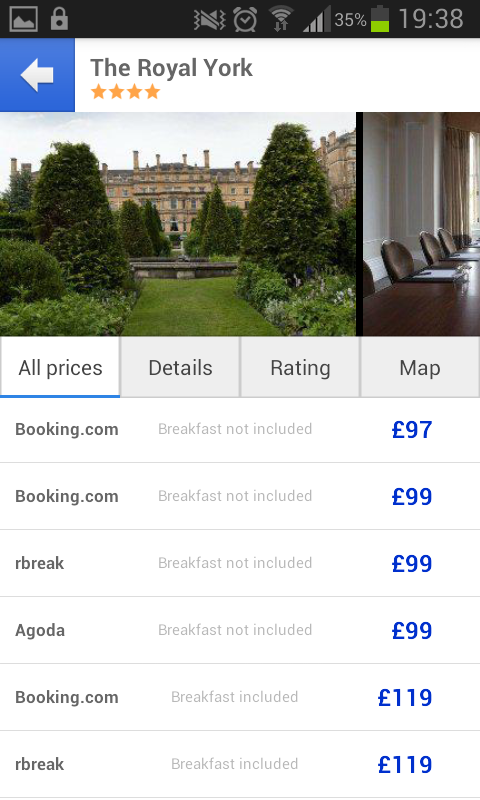
\includegraphics[width=\textwidth]{img/relatedReviews/TrivagoFig3.png}
		\caption{The hotel in more detail}\label{fig:TrivagoFig3}
	\end{subfigure}
	\caption{}\label{fig:trivago2}
\end{figure}

\paragraph{Weaknesses}

\begin{itemize}
	\item The `current location' feature in the search box is useful if you
		need a hotel there and then, but in reality this is rarely the case.
		Customers would usually book a hotel at least a day in advance at which
		point there current location is unlikely to be near an area they would
		need a hotel.
	\item There is no option to select how many people and therefore no option
		for multiple rooms. The user may require multiple rooms if there is
		more than two of them. Therefore this app is useless for families and
		people travelling in large groups.
	\item There are no additional filters past the home screen. Customers may
		require extra filters such as free parking.
\end{itemize}

\subsubsection{thetrainline.com}
\label{ssub:thetrainline}

thetrainline.com is a train ticket retailer app designed to let customers buy
train tickets without the need to have a paper ticket. This app differs
slightly in that it independently searches individual trains without searching
external websites. Train journeys can be searched by location of departure and
destination, departure/arrival  time and number of passengers, as shown in
figure~\ref{fig:theTrainLineFig1}. All available train journeys are then
displayed with the cheapest price for each journey.  Once the customer has
confirmed their chosen journey they can pay for their ticket on
thetrainline.com. The customer will be sent a barcode ticket to their mobile
phone.
% \begin{figure}[htbp]
% 	\centering
% 	\begin{subfigure}[b]{0.2\textwidth}
% 		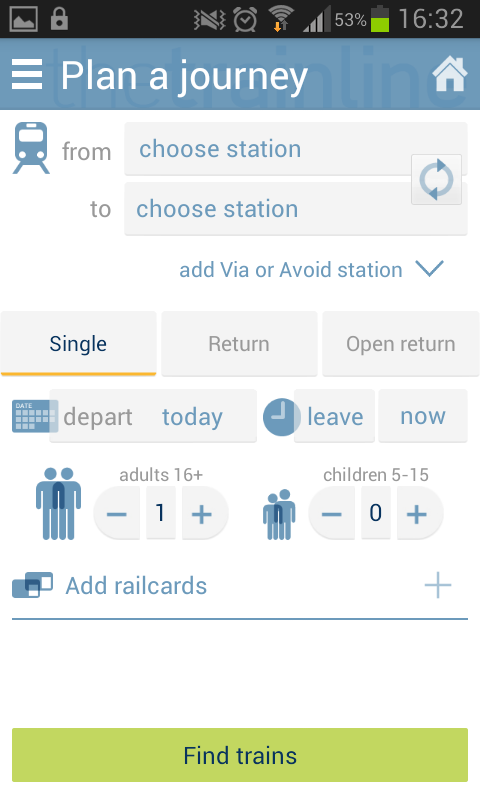
\includegraphics[width=\textwidth]{img/relatedReviews/theTrainLineFig1.png}
% 		\caption{Search criteria screen}\label{fig:theTrainLineFig1}
% 	\end{subfigure}%
% 	\qquad
% 	\begin{subfigure}[b]{0.2\textwidth}
% 		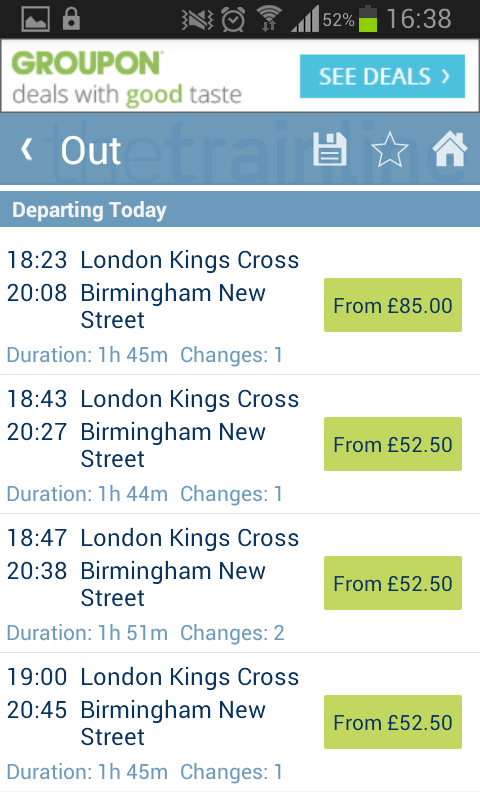
\includegraphics[width=\textwidth]{img/relatedReviews/theTrainLineFig2.png}
% 		\caption{Results from the search}\label{fig:theTrainLineFig2}
% 	\end{subfigure}
% 	\caption{Search using thetrainline.com application.
% 	}\label{fig:thetrainline1}
% \end{figure}
\marginFig[0.8]{img/relatedReviews/theTrainLineFig1.png}{thetrainline search criteria screen}{fig:theTrainLineFig1}
\marginFig[0.8]{img/relatedReviews/theTrainLineFig2.png}{Search results from thetrainline}{fig:theTrainLineFig2}

\paragraph{Strengths}

\begin{itemize}
	\item When typing the name of the station it suggests possible stations
		based on the first few letters. Useful if you're unsure of the name of
		the station. For example, typing `Birmingham' shows a list of all
		stations in Birmingham. In addition to this all recent searches are
		also displayed, so it is not necessary to type the name of the station
		each time.
	\item The app uses GPS to find the customers nearest station and it is also
		possible to set a home station to make it quicker and easier to plan a
		journey home every day (figure~\ref{fig:thetrainline3}).
	\item There is no redirection to another website, the customer can pay
		directly on thetrainline.com which provides a quicker and smoother
		payment process.
	\item The results shown are not limited to the specific time chosen,
		figure~\ref{fig:theTrainLineFig2}. This gives the customer an
		opportunity to choose an earlier or later train if it happens to be a
		lot cheaper.
\end{itemize}
\begin{figure}[htbp]
	\centering
	\begin{subfigure}[b]{0.33\textwidth}
		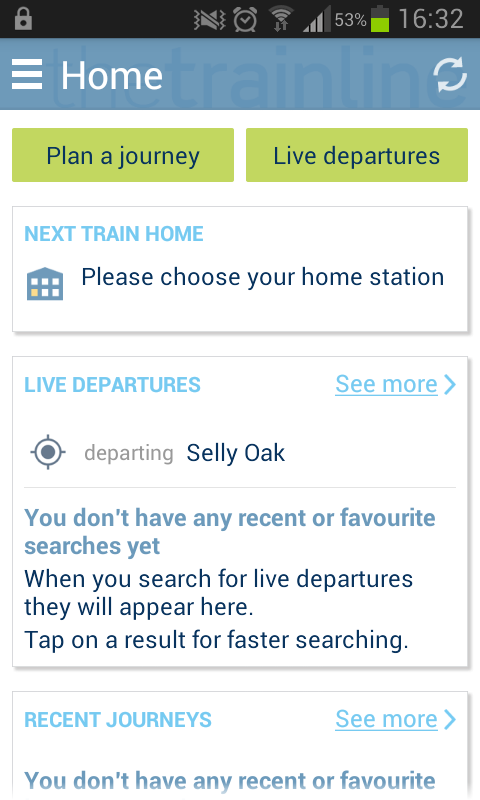
\includegraphics[width=\textwidth]{img/relatedReviews/theTrainLineFig3.png}
		\caption{Home screen showing GPS feature}
	\end{subfigure}%
	\qquad
	\begin{subfigure}[b]{0.33\textwidth}
		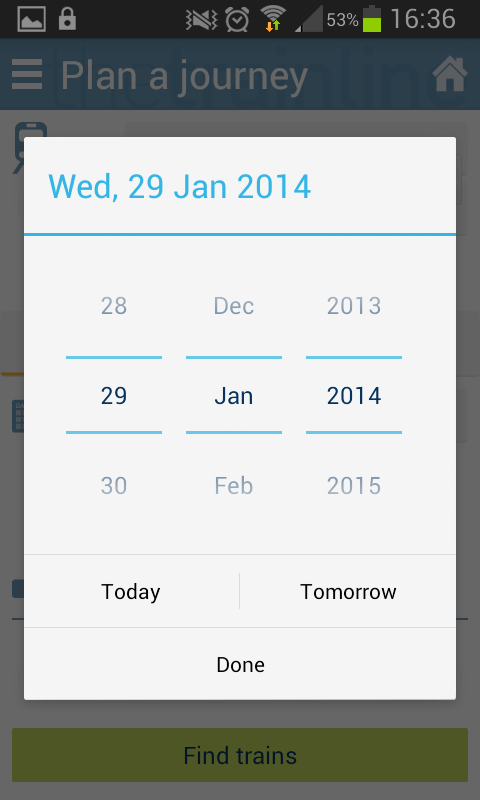
\includegraphics[width=\textwidth]{img/relatedReviews/theTrainLineFig4a.png}
		\caption{Sensitive time selection feature}
	\end{subfigure}
	\caption{}\label{fig:thetrainline3}
\end{figure}

\paragraph{Weaknesses}
\begin{itemize}
	\item The time and date selection feature is very sensitive and therefore
		requires a steady hand when scrolling up and down. The time can also be
		selected to the nearest minute, which when it comes to planning a
		journey, isn't particularly necessary considering multiple journeys are
		shown on the results page. Both these flaws contribute to time taken to
		find the desired journey.
\end{itemize}

\subsubsection{What we can learn}
\label{ssub:what_we_can_learn2}

\begin{itemize}
	\item Our sports booking app would benefit from having a GPS feature as
		those looking to play a particular sport would usually prefer to play
		near their current location. For the same reason, when the results are
		displayed, a filter for distance to the sport venue could be beneficial
		to the user.
	\item It would be useful if a message was sent to the users phone to
		confirm the booking. This will allow the user to check the booking
		details they are likely to forget such as court number or price. If the
		user booked the court well in advance, there could also be an option
		for the user to request  a reminder,  say a day before they are due to
		play.
	\item When searching for a particular location, the user should have the
		option to search by either postcode, address, town or city. By entering
		the city, this gives the user flexibility on location. However if the
		user does not wish to travel far, the other options would be more
		constructive. Either way, there is no restriction on how to search for
		a venue.
\end{itemize}

\subsection{Current Sports Booking Applications}
\label{sub:current_sports_booking_applications}

Our application will allow searching across multiple organisations, locations,
times and sports to provide available bookings. There are currently no
applications that allow searching across multiple organisations' facilities for
available sports bookings. There are, however, web applications for specific
organisations which:
\begin{itemize}
	\item have multiple locations, each with many available sports to play,
	\item have a single location with many sports to play,
	\item have multiple locations with a single sport to play.
\end{itemize}
There are also web applications which allow for searching of different
facilities but offer no information on available bookings beyond providing
contact information for each facility.

\subsubsection{University Of Birmingham Sport}
\label{ssub:university_of_birmingham_sport}

The University Of Birmingham has an online booking system for numerous sports
available to play at facilities at its campus in Edgbaston\cite{UOBSport}. This
site allows search by location, type of activity and time. Once the user has
entered their search criteria, a list of ``activities'' are returned. The user
then selects an activity and is shown a timetable indicating at what time this
activity is available. The activity can then be booked directly on the website.
\begin{figure}[ht]
	\centering
	\begin{subfigure}[b]{0.4\textwidth}
		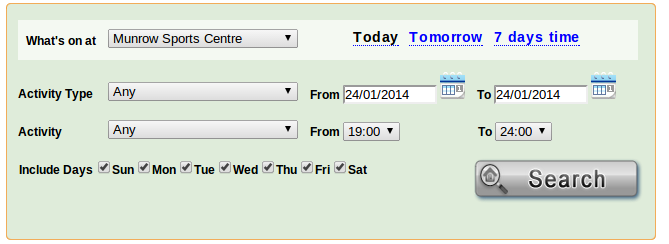
\includegraphics[width=\textwidth]{img/relatedReviews/UoBSearch.png}
		\caption{Search form}\label{fig:UoBSearch}
	\end{subfigure}%
	\qquad
	\begin{subfigure}[b]{0.4\textwidth}
		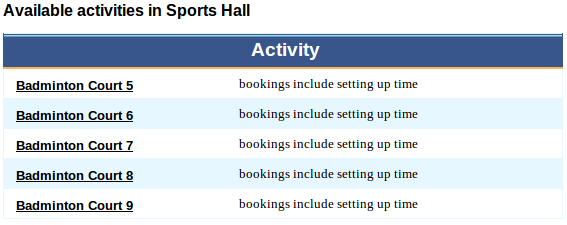
\includegraphics[width=\textwidth]{img/relatedReviews/UoBResults.png}
		\caption{List of results}\label{fig:UoBResults}
	\end{subfigure}
	\qquad
	\begin{subfigure}[b]{0.7\textwidth}
		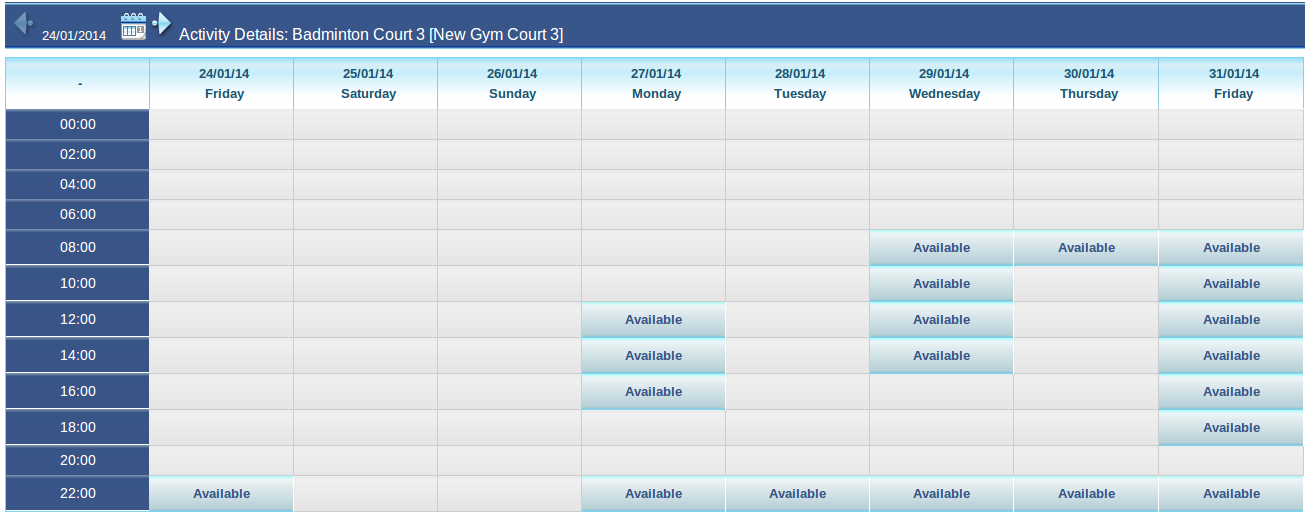
\includegraphics[width=\textwidth]{img/relatedReviews/UoBTimetable.png}
		\caption{Timetable of available bookings}\label{fig:UoBTimetable}
	\end{subfigure}
	\caption{The booking interface for University of Birminghan Sport.
	}\label{fig:animals}
\end{figure}

\paragraph{Strengths}
\begin{itemize}
	\item The search form has tick boxes to filter out particular days of the
		week. A user may only know which days of the week they want to play a
		sport rather than exact dates. This feature gives the user a quick way
		to search for this.
	\item There are quick links on the form to change the date ranges to either
		today, tomorrow or 7 days time. When a group finishes playing a
		particular sport one week, they may want to quickly see what is
		available at the same time the following week; these quick links speed
		up the process of finding these available bookings.
	\item It is possible to search solely by time, leaving all sport and
		location fields blank. If the user knows they want to play a sport at a
		particular time, but would like to have options on sport and location,
		the search form in figure~\ref{fig:UoBSearch} allows them to search
		this way.
\end{itemize}

\paragraph{Weaknesses}
\begin{itemize}
	\item The option to filter by ``activity type'' in the search form is
		actually a filter for location and many of the locations host a variety
		of different sports. Furthermore, the names of these locations, such as
		``Sports Hall'', often offer no clear indication of which sports are
		available at a particular location. If the user wants to know what
		sports are played at a particular venue, they have select that venue
		and then see which options then appear under the ``Activity'' drop down
		box of the search form. This is confusing and unintuitive for the user.
	\item For many sports, such as badminton where there are multiple courts
		available for badminton across several locations, there is no way to
		simply search by that sport. The user is required to go to each court
		individually to see what times are available for that court. The user
		is unlikely to have a court preference and most likely just wants to
		know at what times they can play badminton; this system offers no quick
		and easy way to do this.
	\item The timetable results groups times into two hour slots but often each
		booking slot is one hour long. It will show `available' for a two hour
		slot when at least one of those two hours is available. Therefore it is
		impossible to know if the exact hour a user wants to play is available
		without selecting the containing two hour slot as shown in
		figure~\ref{fig:UoBTimetableDD}.
		\begin{figure}
			\begin{center}
				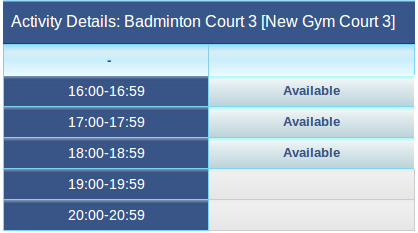
\includegraphics[width=0.4\textwidth]{img/relatedReviews/UoBTimetableDD}
			\end{center}
			\caption{Display when the 18:00 two hour slot is chosen. However,
				only one of two hours following 18:00 is available.
			}\label{fig:UoBTimetableDD}
		\end{figure}

	\item There is no indication of price until you select a booking slot for a
		particular sport at a particular time.
\end{itemize}

\newpage

\subsubsection{Aquaterra Leisure Centres}
\label{ssub:aquaterra_leisure_centres}

Aquaterra is a charity funded by Islington Council who manage several leisure
centres and other sports facilities in Islington, London. They maintain a
website\cite{AquaterraLeisure} where users are able to book at each of these
facilities. The booking home page shown in figure~\ref{fig:AquaterraHome}
prompts a user to select which of the locations they would like to make a
booking at.
\begin{figure}[ht]
	\centering
	\begin{subfigure}[b]{0.3\textwidth}
		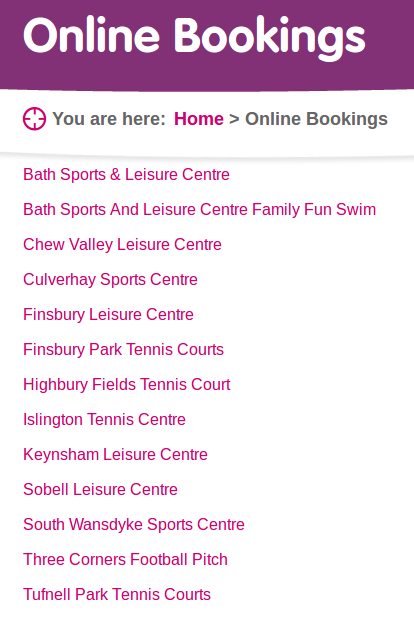
\includegraphics[width=\textwidth]{img/relatedReviews/AquaterraHome.png}
		\caption{Aquaterra booking homepage}\label{fig:AquaterraHome}
	\end{subfigure}
	\qquad
	\begin{subfigure}[b]{0.3\textwidth}
		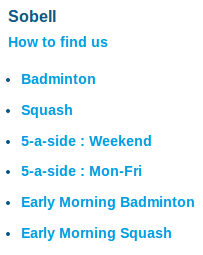
\includegraphics[width=\textwidth]{img/relatedReviews/AquaterraSobellHome.png}
		\caption{Facilities available at Sobell Leisure Centre.
		}\label{fig:AquaterraSobellHome}
	\end{subfigure}
	\qquad
	\caption{The booking interface for Aquaterra Leisure Centres.
	}\label{fig:AquaterraHomeMain}
\end{figure}

The interface for each of the locations varies slightly, but each will
generally show a list of available activities at that location that can be
selected to display a timetable of available booking slots within the following
week for that particular activity. The price is displayed at this point and the
booking can then be made directly on the website after choosing a preferred
court.
\begin{figure}[ht]
	\centering
	\begin{subfigure}[b]{0.4\textwidth}
		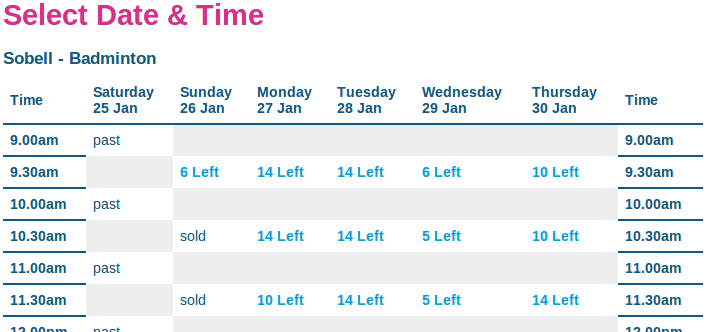
\includegraphics[width=\textwidth]{img/relatedReviews/AquaterraSobellBadminton.png}
		\caption{Beginning of timetable showing available badminton
		slots}\label{fig:AquaterraSobellBadminton}
	\end{subfigure}
	\qquad
	\begin{subfigure}[b]{0.4\textwidth}
		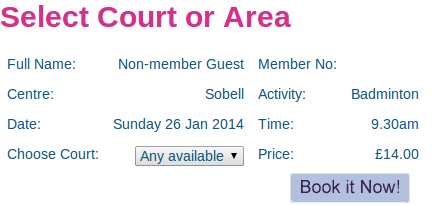
\includegraphics[width=\textwidth]{img/relatedReviews/AquaterraSobellConfirm.png}
		\caption{Confirmation page for a booking slot showing price and choice
		of courts available}\label{fig:AquaterraSobellConfirm}
	\end{subfigure}
	\qquad
	\caption{The booking interface for badminton at Sobell Leisure
	Centre}\label{fig:AquaterraSobellBadmintonMain}
\end{figure}

\paragraph{Strengths}
\begin{itemize}
	\item If a user knows the location they wish to play at and the sport they
		wish to play,  then they can see on one page everything that is
		available to them in the next week. Rows being coloured alternately and
		having the time displayed at both sides of the timetable makes it easy
		for the user to navigate to a particular time slot at a glance.
	\item The timetable for badminton in
		figure~\ref{fig:AquaterraSobellBadminton} indicates how many courts are
		available within each slot. If very few courts are available in a
		preferred time slot, it could indicate to the user that they need to
		make a quick decision as those courts may soon be booked by someone
		else. Conversely, if there are many courts available it could indicate
		to the user that they could delay making a decision on which time to
		book a court. Providing the user with this information early in the
		search process could be very helpful.
\end{itemize}

\paragraph{Weaknesses}
\begin{itemize}
	\item When selecting a location from the page in
		figure~\ref{fig:AquaterraHome}, there is very little indication to the
		user what sports are available at which location. Therefore if they
		want to play a particular sport but have no location preference, they
		are required to go through each option on the homepage to compare what
		facilities are available for that sport at each location. Furthermore,
		as each location's page has a slightly different interface, the user
		has to make sense of each page separately, slowing down their ability
		to compare information provided for each location.
	\item There is no indication of price until you select a particular sport
		at a particular time.
\end{itemize}

\newpage

\subsubsection{London Tennis}
\label{ssub:london_tennis}

London Tennis is a website designed to help tennis players in London find
partners to play with, as well as tournaments to play in and courts to play at.
The court search feature in figure~\ref{fig:LondonTennisSearch} allows a user
to search for a court anywhere in London including options to search by cost of
playing, location and type of court.
\begin{figure}[ht]
	\centering
	\begin{subfigure}[b]{0.6\textwidth}
		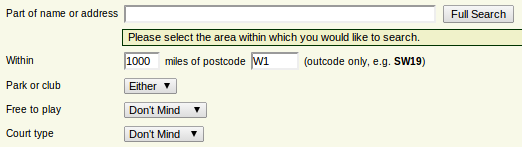
\includegraphics[width=\textwidth]{img/relatedReviews/LondonTennisSearch.png}
		\caption{The search form for looking for a tennis court.
		}\label{fig:LondonTennisSearch}
	\end{subfigure}%
	\qquad
	\begin{subfigure}[b]{0.35\textwidth}
		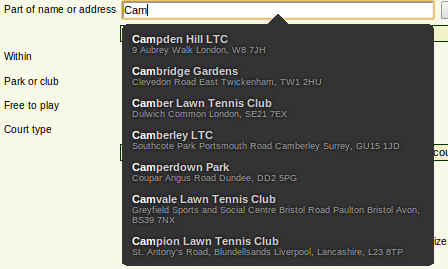
\includegraphics[width=\textwidth]{img/relatedReviews/LondonTennisPredict.png}
		\caption{Drop down to predict input when typing a name of a court.
		}\label{fig:LondonTennisPredict}
	\end{subfigure}
	\qquad
	\caption{The search form for London Tennis.
	}\label{fig:LondonTennisSearchMain}
\end{figure}

There is also the option to select courts from a map, as shown in
figure~\ref{fig:LondonTennisMap}. Users can filter out courts which are free or
not free. However, there are no other interactive features on this map. Once a
search is performed, the user is shown a list of courts matching their chosen
criteria as seen in figure~\ref{fig:LondonTennisResults}. Once a court is
chosen, the user is shown details about the court including exact location,
type of court, price and weather predictions for the local area.
\begin{figure}
	\begin{center}
		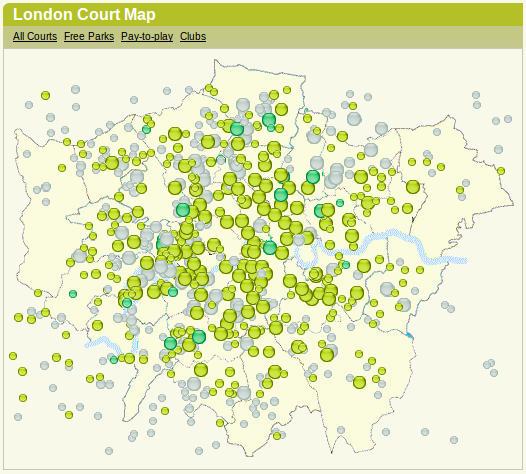
\includegraphics[width=0.7\textwidth]{img/relatedReviews/LondonTennisMap.png}
	\end{center}
	\caption{All courts by location on a map with the ability to filter between
	free and pay-to-play courts}\label{fig:LondonTennisMap}
\end{figure}

\begin{figure}[ht]
	\centering
	\begin{subfigure}[b]{0.7\textwidth}
		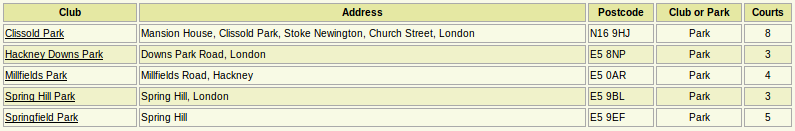
\includegraphics[width=\textwidth]{img/relatedReviews/LondonTennisResults.png}
		\caption{List of courts matching a search.
		}\label{fig:LondonTennisResults}
	\end{subfigure}
	\begin{subfigure}[b]{0.7\textwidth}
		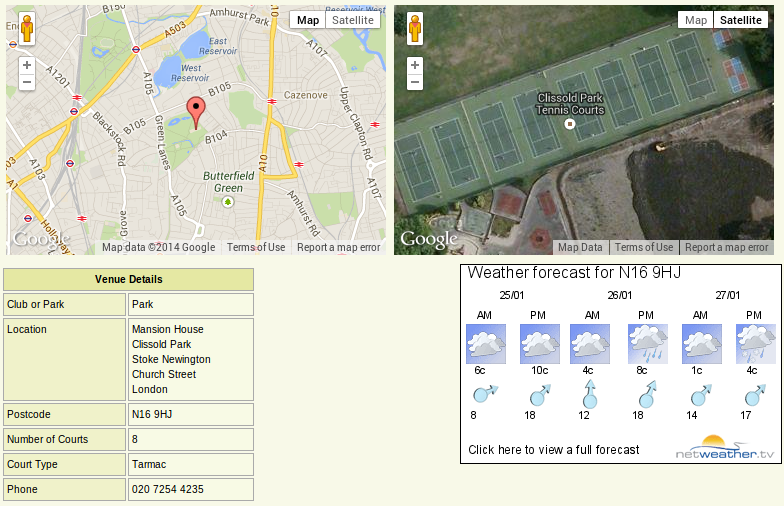
\includegraphics[width=\textwidth]{img/relatedReviews/LondonTennisDetails.png}
		\caption{Details about a chosen court. }\label{fig:LondonTennisDetails}
	\end{subfigure}
	\caption{The displays for results of a search.
	}\label{fig:LondonTennisResultsMain}
\end{figure}

\paragraph{Strengths}
\begin{itemize}
	\item The user is able to show only free courts straight away without
		having to complete any other aspects of the search. This is in contrast
		to other sites we have seen so far and allows the user to immediately
		filter by something that is potentially a deciding factor in choosing a
		court.
	\item The weather predictions are a useful addition given tennis is very
		much dependent on good weather.
\end{itemize}

\paragraph{Weaknesses}
\begin{itemize}
	\item The size of the map for searching in figure~\ref{fig:LondonTennisMap}
		is too small for the number of courts shown on the map, particularly
		given there is no option to zoom in to more detail on the map. Though
		the map does give, at a glance, an idea of where courts are
		concentrated in London, it is difficult to actually select a court due
		to how close the buttons to select each court are to each other.
	\item There is no information about opening times for any of the courts.
		Although London Tennis is primarily a service to find court locations
		rather than provide details about available bookings it would be useful
		to inform the user of when the courts are even open.
\end{itemize}

\subsubsection{What we can learn}
\label{ssub:what_we_can_learn}

\begin{itemize}
	\item It could be useful to add options to filter by day of the week in
		addition to buttons that quickly allow searching by times relative to
		today such as tomorrow or one week from now as this is possibly be one
		of the main criterias of the users search.
	\item The naming of options to filter by when searching need to be
		intuitive and unambiguous otherwise it is difficult  for the user to
		know how to actually search for what they want.
	\item Using a timetable layout similar to figure~\ref{fig:UoBTimetable}
		could create difficulties in clearly displaying all available options
		after a search is done. There may be far more booking slots to display
		in our app given that our search will be conducted over a greater
		number of facilities. The screen space available will also be smaller
		than University of Birmingham has on their website. Therefore we need
		to think of a clearer way of showing the user the results of a search.
	\item Price is likely to be a factor in a user's decision of what sport to
		play and where, therefore our application needs to either provide a
		filter to search by price or clearly indicate the price of a booking
		option as early as possible when displaying results to a user.
	\item If we are to use a map to display results of a search, it will be
		difficult given the potentially large number of results to display
		every option individually on the map, particularly if the map covers a
		large area. Therefore it may be better to group options together,
		possibly by colour or different shapes or picture icons, in order to
		make it possible to read and navigate through the results.
	\item Weather could be an important factor when a user knows when they
		would like to play a sport but want to compare what sports are
		available at that time. When a user is looking at search results for
		outdoor bookings, it could be useful to display weather predictions for
		that time, particularly if the search is in the near future as
		predictions are likely to more accurate for the near future.
\end{itemize}

\subsection{Application Considerations}
\label{sub:application_considerations}

Depending on the operating system, each platform has it's own specific
guidelines on how to provide users with a good experience. Key issues include;
page layout, navigation and interaction.
\marginFig{img/relatedReviews/iOS_page}{iOS page layout recommendation}{fig:iOS_page}

Apple recommends that the most important feature of an app should be displayed
at the top-left of the page so that it will be the first thing a user
sees\cite{HIGApple2013}.  Booking.com and the trainline.com both implement this
well\cite{BookingcomIOS}.
\marginFig[0.7]{img/relatedReviews/booking_page}{Booking page for thetrainline.com\cite{thetrainlineIOS}.}{fig:booking_page}
% \begin{figure}[htbp]
% 	\centering
% 	\begin{subfigure}[b]{0.5\textwidth}
% 		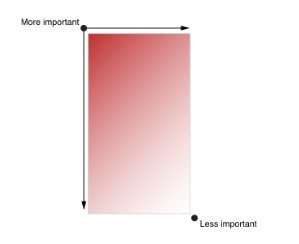
\includegraphics[width=\textwidth]{img/relatedReviews/iOS_page}
% 		\caption{iOS page layout recommendation}\label{fig:iOS_page}
% 	\end{subfigure}%
% 	\qquad
% 	\begin{subfigure}[b]{0.25\textwidth}
% 		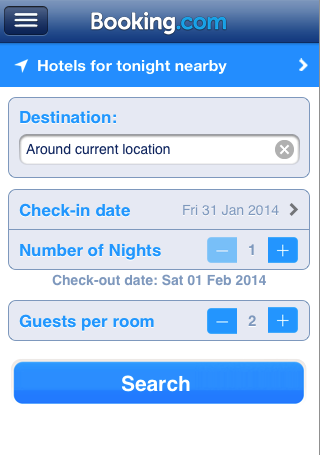
\includegraphics[width=\textwidth]{img/relatedReviews/booking_page}
% 		\caption{Booking page for thetrainline.com\cite{thetrainlineIOS}. }
% 	\end{subfigure}
% 	\caption{}\label{fig:booking_page}
% \end{figure}

Users should be able to navigate their way through the app to achieve their
goal of booking sports facilities.

There are 3 main styles of navigation;
\begin{description}
	\item[Hierarchical] navigation is where users make one choice on the first
		screen, another on the second screen and so on until they reach their
		final destination. To navigate to another destination, the user may
		have to retrace some steps or start over from the beginning. This could
		be very inconvenient for the user as they may have to go back several
		steps or start over.
	\item[Content or Experience-driven] navigation depends on the content of
		the application. The navigation also plays an important part of the app
		experience. The Skyscanner app includes a globe,
		figure~\ref{fig:skyscanner_globe}, which allows the user to explore the
		cost of travelling to particular locations. This is a feature provides
		a unique experience for the user.
		\begin{figure}[htbp]
			\begin{center}
				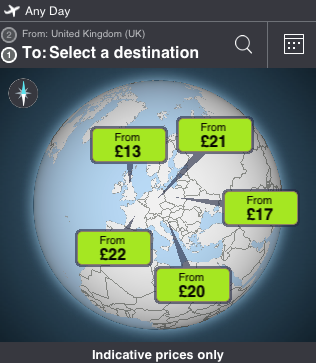
\includegraphics[width=0.4\textwidth]{img/relatedReviews/skyscanner_globe}
			\end{center}
			\caption{Skyscanner apps globe feature}\label{fig:skyscanner_globe}
		\end{figure}

	\item[Flat] navigation allows users are move from one category to another,
		as all categories are available from the main screen. This style has
		been used by many of the apps studied including redspottedhanky.com,
		booking.com and thetrainline.com
		% \begin{figure}[htbp]
		% 	\begin{center}
		% 		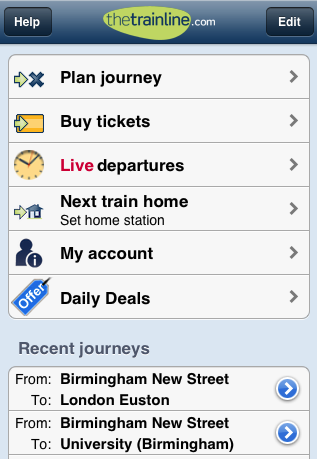
\includegraphics[width=0.25\textwidth]{img/relatedReviews/trainline_main}
		% 	\end{center}
		% 	\caption{Trainline main\cite{thetrainlineIOS}. }\label{fig:trainline_main}
		% \end{figure}
\end{description}

In some cases, it may be better to combine more than one navigation style, but
it could also run the risk of overcomplicating the design of the app and the
user's experience.

Some apps like Trivago have a navigation bar, which manages the screen's
contents. The user can select to change the search criteria or pinpoint hotels
on a map. In the Zipcar app, figure~\ref{fig:zipcar_nav_bar}, the options in
the navigation bar allow the user to perform actions. E.g. `Reserve' or `Log
in'. These options change depending on where the user is in terms of navigation
\begin{figure}[htbp]
	\begin{center}
		
\includegraphics[width=0.45\textwidth]{img/relatedReviews/zipcar_nav_bar1}
		\quad
		
\includegraphics[width=0.45\textwidth]{img/relatedReviews/zipcar_nav_bar2}
	\end{center}
	\caption{Zipcar navigation\cite{ZipCarIOS}.}\label{fig:zipcar_nav_bar}
\end{figure}

Some navigation styles have tab bars placed at the bottom of the screen; this
allows the user to switch between different subtasks, views or modes. For
example, redspottedhanky.com's app includes the options of switching between
finding trains, viewing tickets or account details or finding other
information. This is a useful feature that helps a user navigate their way
through an app, which thetrainline.com has chosen not to use in their design.

Apple and Microsoft both recommend $44\times44$ points and a maximum of 5 icons
to avoid tab bars being over cluttered.
\begin{figure}[htbp]
	\centering
	\begin{subfigure}[b]{0.35\textwidth}
		
\includegraphics[width=\textwidth]{img/relatedReviews/redspottedhanky_tab_bar}
		\caption{RedspottedHanky tab bar. }\label{fig:redspottedhanky_tab_bar}
	\end{subfigure}%
	\qquad
	\begin{subfigure}[b]{0.4\textwidth}
		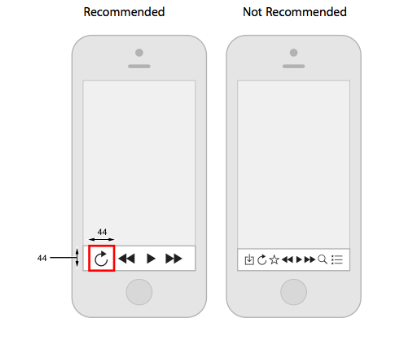
\includegraphics[width=\textwidth]{img/relatedReviews/iOS_tab_bar}
		\caption{iOS tab bar.}\label{fig:iOS_tab_bar}
	\end{subfigure}
	\caption{Tab bar icon sizes.}
\end{figure}

None of the apps studied take into account the orientation of the screen. Users
have no option but to use the apps when the phone is in portrait. It would be
best to provide users with the choice of holding their device in landscape too.
As can be seen in figure~\ref{fig:trivago_input}, Trivago, in particular,
contains a lot of details within its side menu; some users may prefer to see
slightly bigger, which could be possible when the screen is tilted
horizontally.
\marginFig[0.7]{img/relatedReviews/trivago_input}{Trivago input\cite{TrivagoIOS}.}{fig:trivago_input}
% \begin{figure}[htbp]
% 	\begin{center}
% 		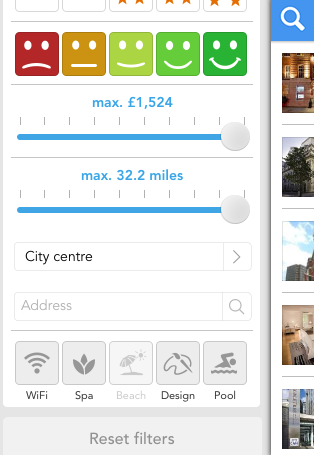
\includegraphics[width=0.25\textwidth]{img/relatedReviews/trivago_input}
% 	\end{center}
% 	\caption{Trivago input\cite{TrivagoIOS}. }\label{fig:trivago_input}
% \end{figure}

The way all of the apps function is through a touchscreen interface. Users may
be used to certain functions such as `pinch to zoom' and other interactions
defined below for iOS\@. It will be important to consider these interactions to
make the app easy to use
\begin{figure}[htbp]
	\centering
	\begin{subfigure}[b]{0.7\textwidth}
		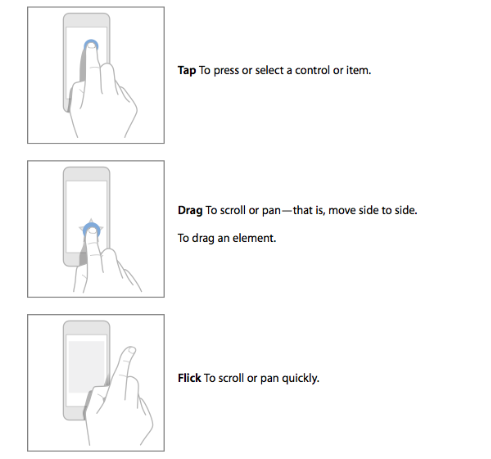
\includegraphics[width=\textwidth]{img/relatedReviews/iOS_touch}
		\caption{iOS touchscreen interactions}\label{fig:iOS_touch}
	\end{subfigure}%
	\qquad
	\begin{subfigure}[b]{0.7\textwidth}
		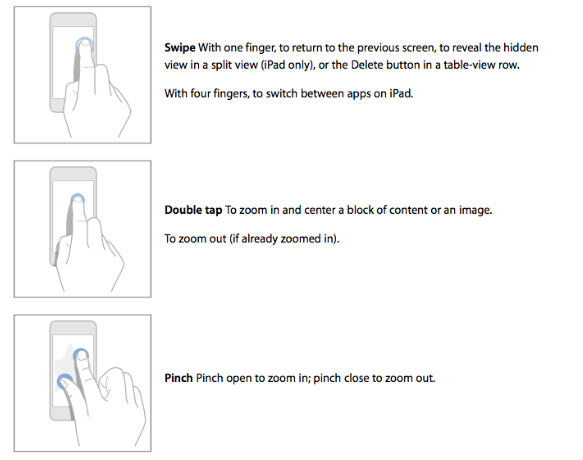
\includegraphics[width=\textwidth]{img/relatedReviews/iOS_touch_2}
		\caption{iOS touchscreen interactions}
	\end{subfigure}
	\caption{}\label{fig:iOS_touch2}
\end{figure}

Other ways the user could provide input include using speech recognition. For
example, the user could say the sport, date, time and location instead of
having to input text or select options.

% subsection application_considerations (end)


% section review_of_related_work (end)

\bibliographystyle{plain}
\bibliography{references}
\end{document}
